\pagenumbering{arabic} %necessary to start numbering pages in arabic numerals from here
\setcounter{page}{1} 

\section{Introducción}
\subsection{Problemática}
La comunicación es un derecho humano fundamental. Sin embargo, personas con discapacidades del lenguaje enfrentan barreras significativas para expresarse. La Comunicación Aumentativa y Alternativa (CAA) ofrece una solución mediante el uso de pictogramas, los cuales son representaciones visuales de conceptos que permiten transmitir mensajes sin depender del lenguaje verbal convencional \cite{beukelman2013}.

El Portal Aragonés de Comunicación Aumentativa y Alternativa (ARASAAC) es uno de los sistemas pictográficos más utilizados a nivel mundial, con más de 12,000 pictogramas de uso libre \cite{arasaac2007}. A pesar de la disponibilidad de estos recursos, la traducción automática de lenguaje natural a secuencias de pictogramas sigue siendo un reto.

Para ilustrar la complejidad del problema, considérese una oración con ambigüedad léxica como: \textit{"El niño se sienta en el banco"}. Un sistema básico de mapeo podría mostrar un pictograma referente a una "institución financiera" en lugar del objeto para sentarse. El objetivo de este trabajo es lograr una traducción que comprenda el contexto global a través del desarrollo de un modelo de aprendizaje profundo unificado. Por ejemplo, ante la entrada: 
\begin{center}
    \textit{"Mañana quiero ir al parque a jugar con mi perro."}
\end{center}
\begin{figure}[htbp]
    \centering
    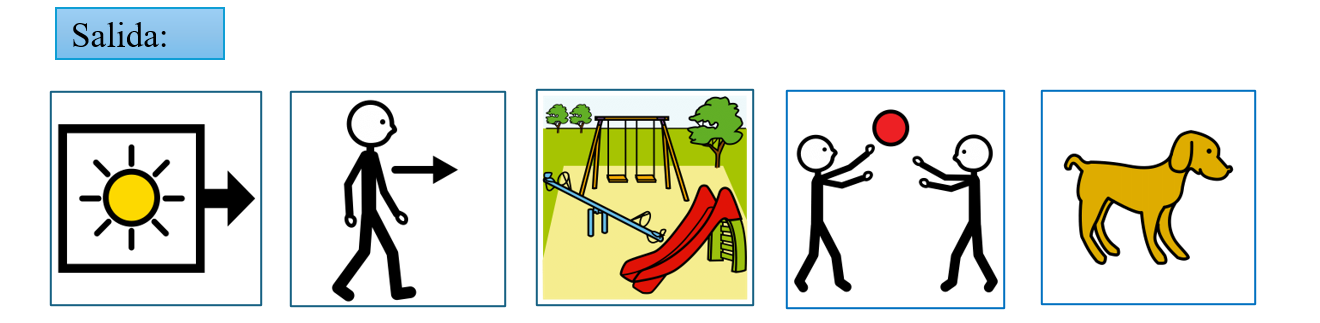
\includegraphics[width=0.75\textwidth]{img/ejemplo1.png}
    \caption{Ejemplo de secuencia de pictogramas}
    \label{fig:ejemplo de salida}
\end{figure}
El sistema no solo debe buscar las imágenes individuales que corresponden a cada palabra, sino sintetizar de forma óptima la estructura gramatical para presentar una secuencia coherente de pictogramas (véase la Figura~\ref{fig:ejemplo de salida}) que mantenga la intención semántica original del usuario.
\subsection{Justificación}
La comunicación constituye un derecho humano fundamental, sin embargo, su ejercicio pleno permanece inaccesible para las  personas que presentan discapacidades del lenguaje derivadas de condiciones como el autismo, la afasia, el síndrome de Rett o la parálisis cerebral. En México, el Instituto Nacional de Estadística y Geografía estima que más de más de 900 mil personas tienen una discapacidad para hablar o comunicarse \cite{inegi2020cpv}, por tal motivo es relevante desarrollar herramientas tecnológicas de apoyo accesibles y eficaces. La Comunicación Aumentativa y Alternativa (CAA), particularmente mediante el uso de pictogramas, representa una de las vías más consolidadas para atender esta necesidad \cite{beukelman2013}.

No obstante, los sistemas actuales de traducción automática de texto a pictogramas presentan limitaciones estructurales que restringen considerablemente su utilidad práctica. Herramientas como AraWord operan mediante mapeo léxico directo, ignorando el contexto de la oración \cite{araword2020}. Por su parte,  Text-to-Pictogram incorpora redes léxicas y técnicas de desambiguación de sentidos, pero pierde la coherencia global al procesar el texto de forma lineal y modular \cite{sevens2015}. Otra herramienta para este propósito, Aratraductor, si bien dio un paso importante al usar análisis sintáctico  para identificar lemas y  usar una técnica de N-grams para detectar frases hechas; este enfoque depende demasiado de reglas gramaticales fijas, lo cual impide su generalización y escalabilidad. Ninguno de estos enfoques es capaz de modelar de forma integral las dependencias semánticas de una oración, tampoco de manejar adecuadamente fenómenos como la polisemia, la negación o las expresiones idiomáticas. La raíz de estas deficiencias reside en su arquitectura: al ser sistemas modulares basados en reglas o recursos lingüísticos explícitos, carecen de la capacidad de aprender representaciones contextuales a partir de datos.

\subsection{Solución propuesta}
Frente a este panorama, el presente trabajo propone una arquitectura de aprendizaje profundo unificada, fundamentado en la arquitectura Transformer \cite{vaswani2017attention}. A diferencia de los modelos precedentes, esta aproximación aprovecha el mecanismo de \textit{self-attention} para modelar dependencias globales en la oración, permitiendo que la generación de cada pictograma considere el contexto semántico completo y no solo la unidad léxica inmediata. La adopción de modelos pre-entrenados como T5 o mT5 \cite{raffel2020}  permite transferir conocimiento lingüístico profundo hacia la tarea específica de traducción a pictogramas. La originalidad de la propuesta reside en dos ejes: la aplicación de arquitecturas Transformer para el modelado integral del contexto, y la validación mediante un diseño experimental que emplea métricas estandarizadas de traducción automática. Esto permitirá realizar una comparativa objetiva entre el enfoque propuesto y los sistemas tradicionales basados en reglas.

El sistema beneficiaría directamente a personas usuarias de CAA y a sus familias, cuidadores y terapeutas del lenguaje, así como a desarrolladores de aplicaciones de accesibilidad, e incluso a personas aprendiendo un segundo idioma. Su viabilidad es alta,  por la disponibilidad abierta de los pictogramas ARASAAC, así como también por el aporte del corpus en inglés de la tarea \textit{Text-to-Picto} de ImageCLEF 2026. ImageCLEF es un laboratorio de evaluación internacional que forma parte de la CLEF (Conference and Labs of the Evaluation Forum), una iniciativa europea centrada en la evaluación de sistemas de información, se lleva a cabo cada año desde 2003 \cite{unknown-author-no-date2}.

Desde una perspectiva académica, el proyecto abarca distintas áreas relevantes de la Ingeniería en Inteligencia Artificial. Lo anterior se logra al establecer un flujo de trabajo estructurado donde el procesamiento de lenguaje natural se usa para preparar los datos; luego apoyándose en el aprendizaje profundo, se entrena a un modelo Transformer, y finalmente las métricas de evaluación validan el éxito de los resultados. Al trabajar estas áreas como un conjunto unificado, el proyecto busca resultados técnicos confiables y un beneficio social real.

\subsection{Objetivo general}

Desarrollar un sistema de traducción automática de texto en lenguaje natural a secuencias de pictogramas ARASAAC, basado en arquitecturas de aprendizaje profundo (Transformers).





\subsection{Objetivos particulares}
\begin{enumerate}
    \item Construir un corpus  Español-Pictogramas a partir de los datos de la tarea \textit{Text-to-Picto} de ImageCLEF 2026, realizando la traducción  y la validación de la alineación semántica para el idioma español.
    \item Implementar un modelo \textit{encoder-decoder} basado en Transformers para la tarea de traducción texto a pictogramas.
    \item Evaluar el sistema propuesto utilizando métricas estándar de traducción automática.
    \item Desarrollar una interfaz de usuario web que consuma el modelo entrenado mediante una API, permitiendo la interacción en tiempo real y la visualización de las secuencias generadas.
\end{enumerate}


\subsection{Metodología}

La metodología del proyecto seguirá de manera adaptada y práctica las fases del modelo \textit{CRISP-ML}, orientadas a garantizar calidad, trazabilidad y reproducibilidad en el desarrollo de un sistema de traducción automática de texto a pictogramas. Cada fase indica las actividades, entregables y controles de calidad asociados.

\begin{enumerate}

    \item \textbf{Comprensión del problema y de los datos (\textit{Business \& Data Understanding})}

    En una primera etapa, se definirá con claridad el problema desde una perspectiva técnica y social. Se establecerán los objetivos funcionales del sistema, determinando que el modelo deberá traducir texto en español, y en otros cuatro idiomas (inglés, alemán, ruso y turco), a secuencias coherentes de identificadores de pictogramas de ARASAAC, preservando el significado semántico global del mensaje. En esta fase se evaluarán también los conjuntos de datos disponibles para la tarea y se seleccionará el que se ajuste al alcance del proyecto.

    Asimismo, se especificarán criterios de éxito medibles, tales como desempeño en métricas automáticas (\textit{SacreBLEU}, \textit{METEOR}, \textit{PictoER}), reducción de ambigüedades léxicas y tiempos de respuesta aceptables en la \textit{API} de inferencia. También se establecerán requisitos no funcionales relacionados con accesibilidad y reproducibilidad.

    \item \textbf{Ingeniería de datos (\textit{Data Engineering / Data Preparation})}

    Se partirá del corpus \textit{Propicto-Orfeo}, cuyos textos fuente en francés se traducirán a cinco idiomas con NLLB-200. Antes de traducir el corpus completo se verificará la calidad de la traducción mediante una prueba piloto evaluada con CometKiwi. Cada ejemplo se procesará de forma bidireccional (texto a identificadores e identificadores a texto). Posteriormente, se definirán dos configuraciones de vocabulario: una que conserva el tokenizador original del modelo y otra que agrega como tokens completos los identificadores de pictograma frecuentes.

    En paralelo, se definirá el vocabulario de salida correspondiente a los identificadores de pictogramas ARASAAC. Se estructurará el corpus en particiones de entrenamiento, validación y prueba, garantizando que todas las versiones de una misma oración (sus cinco traducciones y ambas direcciones) pertenezcan a la misma partición, para evitar filtraciones de información.

    \item \textbf{Ingeniería del modelo de aprendizaje automático (\textit{Machine Learning Model Engineering})}

    En la fase de modelado se ajustará un modelo de lenguaje \textit{decoder-only} preentrenado y multilingüe (Qwen3-4B) mediante LoRA, una técnica de ajuste eficiente que entrena solo un pequeño conjunto de parámetros adicionales. El modelo aprenderá a predecir directamente la secuencia de identificadores de pictogramas a partir del texto. Se compararán las dos configuraciones de vocabulario definidas en la fase anterior.

    Se establecerán configuraciones experimentales que incluirán selección de hiperparámetros, optimizador, tasa de aprendizaje y estrategias de regularización. Se utilizará validación temprana para prevenir sobreajuste y se almacenarán los pesos correspondientes a los mejores modelos obtenidos.

    Adicionalmente, se utilizará como línea base el traductor basado en reglas empleado en la construcción del corpus, con el fin de establecer una referencia cuantitativa que permita demostrar las mejoras aportadas por el enfoque neuronal.

    \item \textbf{Evaluación de los modelos (\textit{Evaluating Machine Learning Models})}

    El sistema entrenado será evaluado utilizando métricas estándar de traducción automática como \textit{SacreBLEU}, \textit{METEOR} y \textit{PictoER}. Las métricas se calcularán sobre las secuencias de identificadores de pictograma y, para comparar con los sistemas de ToPicto 2026, también sobre los términos obtenidos al convertir los identificadores mediante el léxico de ARASAAC.

    Los resultados se compararán con la línea base de reglas y con los sistemas reportados en ToPicto 2026, considerando que el modelo propuesto es de mayor tamaño, lo que limita la atribución de las mejoras únicamente al enfoque. A partir de esta comparación se establecerá una discusión crítica sobre ventajas y limitaciones del enfoque propuesto.

    \item \textbf{Despliegue (\textit{Deployment})}

    Una vez validado el modelo, se procederá a su integración en una arquitectura de servicio. El modelo será encapsulado en una \textit{API REST} que permitirá recibir texto en cualquiera de los cinco idiomas del corpus, generar directamente la secuencia de identificadores de ARASAAC y validar que existan en su catálogo.

    Posteriormente, se desarrollará una interfaz web que consumirá dicha \textit{API}, permitiendo al usuario introducir texto y visualizar de forma inmediata los pictogramas generados. La interfaz priorizará criterios de accesibilidad y claridad visual, asegurando facilidad de uso para usuarios finales. Las imágenes se obtendrán del servicio de ARASAAC y conservarán la atribución que exige su licencia CC BY-NC-SA.

    El sistema será empaquetado mediante tecnologías de contenedorización, lo que permitirá su despliegue reproducible en distintos entornos.

    \item \textbf{Monitoreo y mantenimiento (\textit{Monitoring and Maintenance})}

    Se monitoreará el modelo durante un periodo determinado para verificar su correcto funcionamiento mediante el análisis de métricas de desempeño, incluido el porcentaje de identificadores generados que no existen en el catálogo de ARASAAC. En caso de detectar anomalías o degradación en el rendimiento, se realizará el mantenimiento correspondiente.

\end{enumerate}

\subsection{Estructura del trabajo}